\documentclass[main.tex]{subfiles}

\begin{document}

\section{Description of the simulation}

Use LAMMPS to make a 3D simulation of a binary mixture of two types of particles interacting through a Lennard-Jones force. 
Type 1 particles should have a radius of $1\sigma$ and type 2 should have a radius of $2\sigma$. The particles are connected to a bath, and therefore have a Langevin thermostat.

Use OVITO to visualize the results of the simulation. Make an animation, for three different values of the density, trying to get qualitatively different behaviors. Also make a report where you show a snapshot of the animation and discuss your results. 

\subsection{Langevin thermostat}

According with \cite{Langevin_equation} the Langevin equation provided a conceptual and quantitative improvement on the description of the phenomenon of Brownian motion.
This equation is a stochastic differential equation written as follows
\begin{gather}
    d\upsilon\qty(t) = -\gamma\upsilon\qty(t)+Ddw\qty(t),
\end{gather}
where $\upsilon\qty(t)$ is the velocity, $\gamma$ is a friction coefficient due to the viscosity of the liquid, $D$ is the diffusion coefficient and $w\qty(t)$ is the Wiener process.
Finally, the friction coefficient $\gamma$ and the diffusion coefficient $D$ are related by: $D=2\gamma kT$, where $k$ is the Boltzmann's constant and $T$ is temperature.

This equation can be interpreted as the description of a heavy particle moving through a solvent.
While is moving it will encounter more solvent particles in the front than in the back.
Therefore, the collisions with the solvent particles will on average have the effect of a friction force proportional and opposite to the velocity of the heavy particle \cite{libroClase}.
However, the solvent is modeled by a stochastic and dissipative force, allowing substantially longer simulations that would be possible if the solvent were explicitly included \cite{Luckhurst_Veracini_2012}.

In the following section is a brief description of the software LAMMPS and how it was set the simulation for a binary mixture with Lennard-Jones force and langevin thermostat.

\subsection{LAMMPS}

LAMMPS is an acronym for Large-scale Atomic/Molecular Massively Parallel Simulator and on the LAMMPS website it describes its program as a classical molecular dynamics code with a focus on materials modeling and  has potentials for solid-state materials (metals, semiconductors) and soft matter (biomolecules, polymers) and coarse-grained or mesoscopic systems. 
It can be used to model atoms or, more generically, as a parallel particle simulator at the atomic, meso, or continuum scale \cite{LAMMPS}.

For the simulation of the binary mixture a tutorial by Simon Gravelle \cite{Gravelle}.
The objective of that tutorial is to set set, launch and analyze a molecular dynamics simulations of a binary Lennard-Jones fluid made of neutral particles with two different diameters in a cubic box with periodic boundary conditions and the temperature if the system is imposed using a Langevin thermostat.
In the following sections are shown the results from the simulations.

\section{Results}

In figure \ref{fig:initialCondiitons} is shown a snapshot of the initial conditions for the binary mixture displayed using Ovito.
As it is shown in the figure the particles are set up at a random position inside the box.
At setting this configuration as the initial condition is necessary to run a minimization procedure before initialize the molecular dynamics to prevent the simulation from diverging.

\begin{figure}[ht]
    \centering
    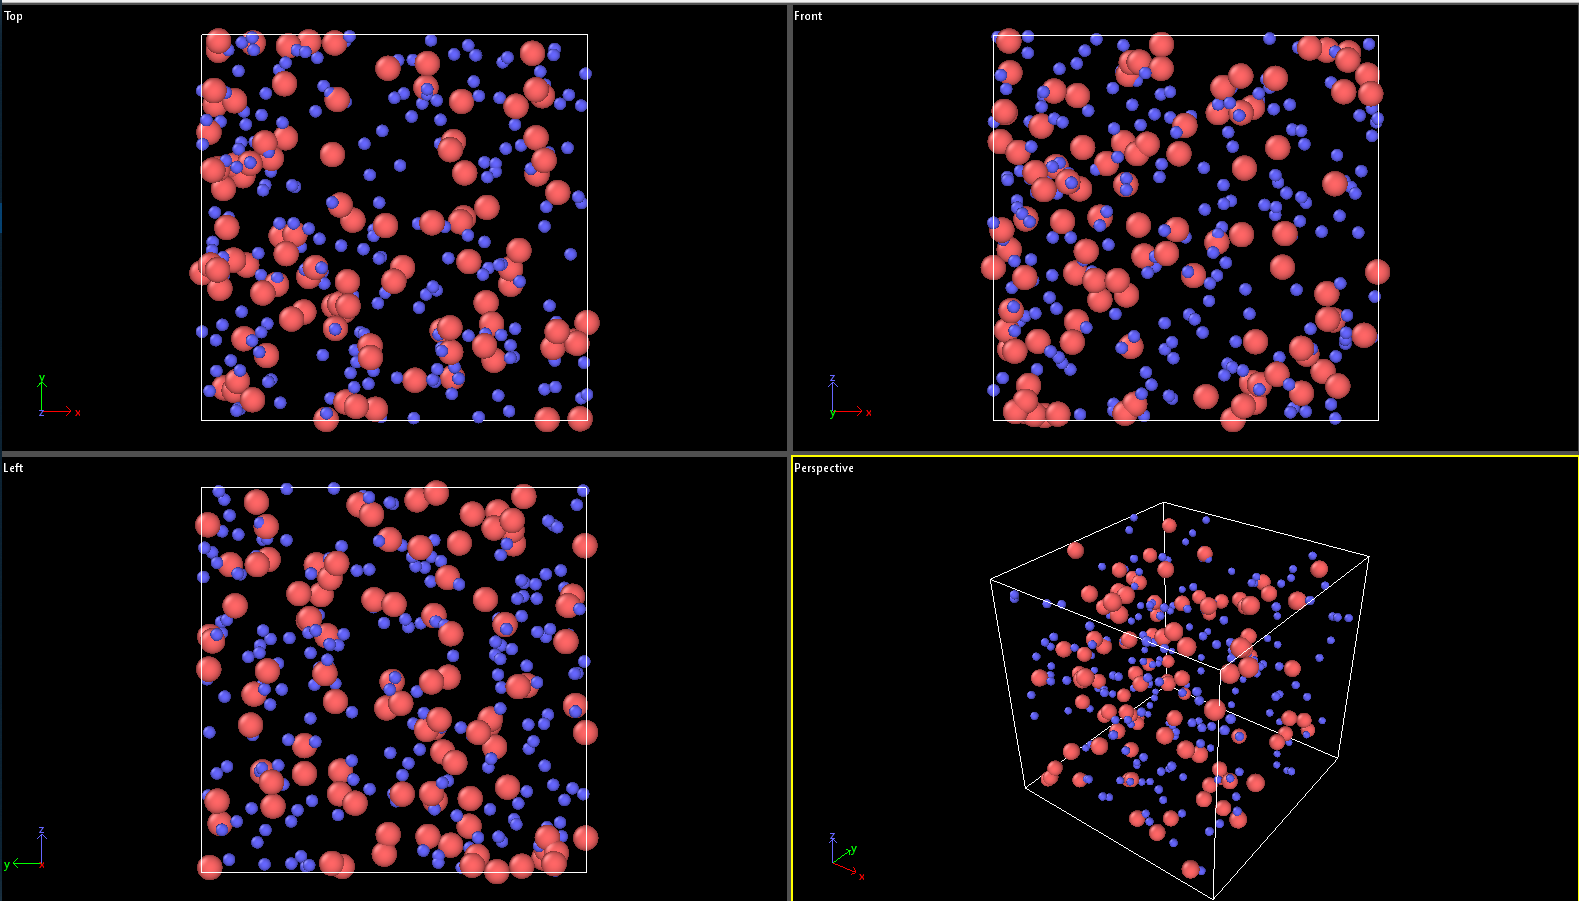
\includegraphics[width=0.8\textwidth]{imgs/hw3/InitialConditions.png}
    \caption{Snapshot of the initial conditions viewed in Ovito.}
    \label{fig:initialCondiitons}
\end{figure}

From the simulation is retrieved the temperature, potential, kinetic and total energy of the system as a tool to analyze the simulation.
In figure \ref{fig:temp} is shown the evolution of the temperature thru the time steps and it is observed that converges to a value, indicating a stable system.
Also in figure \ref{fig:energy}, are shown the potential, kinetic and potential energy of the system thru all the simulation.
As expected, the kinetic energy has a similar curve as the temperature, tending towards a constant value.
On the other hand, the potential energy can be neglect from the total energy, due to the difference in magnitude with the kinetic energy.

Finally in appendix \ref{subsec:script} is the script used for the simulation and in the following link is the access to the animation of the system:
\href{https://tecmx-my.sharepoint.com/:i:/g/personal/a00827546_tec_mx/Edb0vAaSVpNMnYdZ_XIKdA0B2H9gE0njt1jfPwtb59KdlA?email=leogabac%40tec.mx&e=NaACb8}{\color{blue}{Access to the animation}}


\begin{figure}[ht]
    \centering
    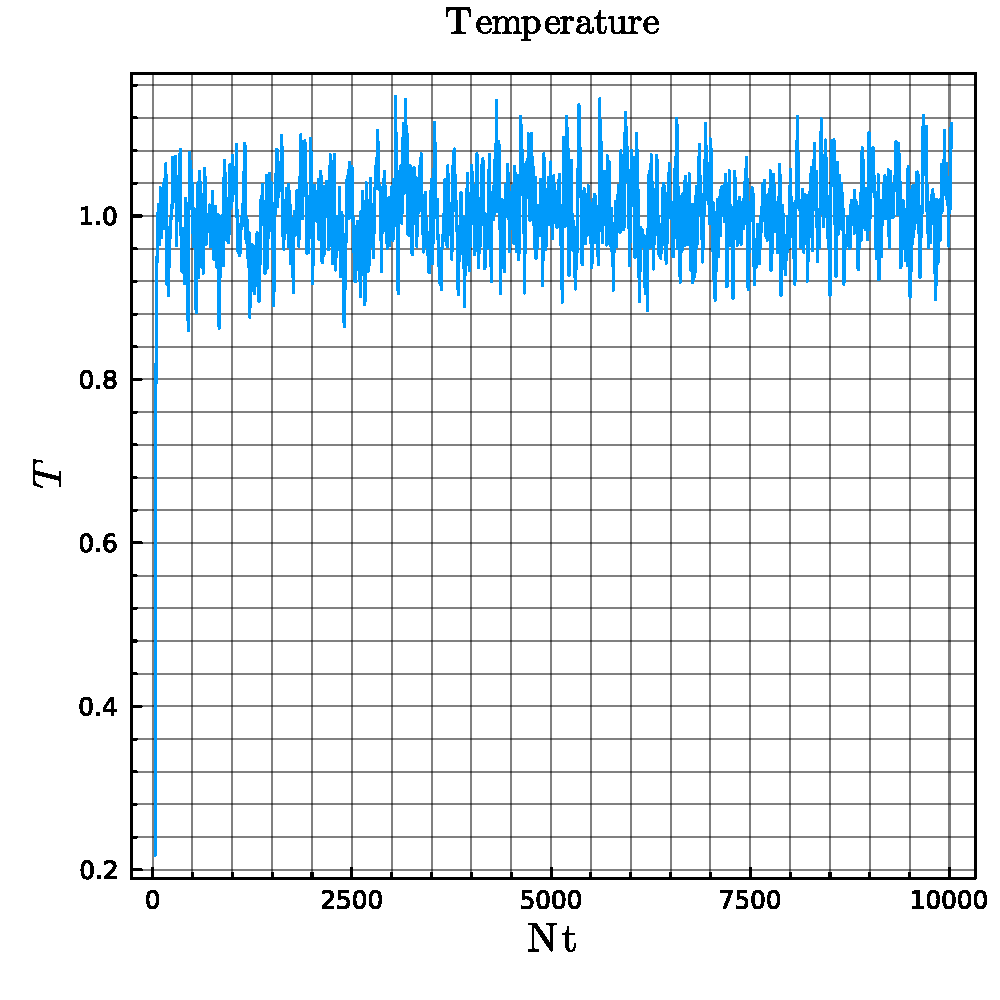
\includegraphics[width=0.65\textwidth]{imgs/hw3/temperature.pdf}
    \caption{Temperature of the system}
    \label{fig:temp}
\end{figure}

\begin{figure}[ht]
    \centering
    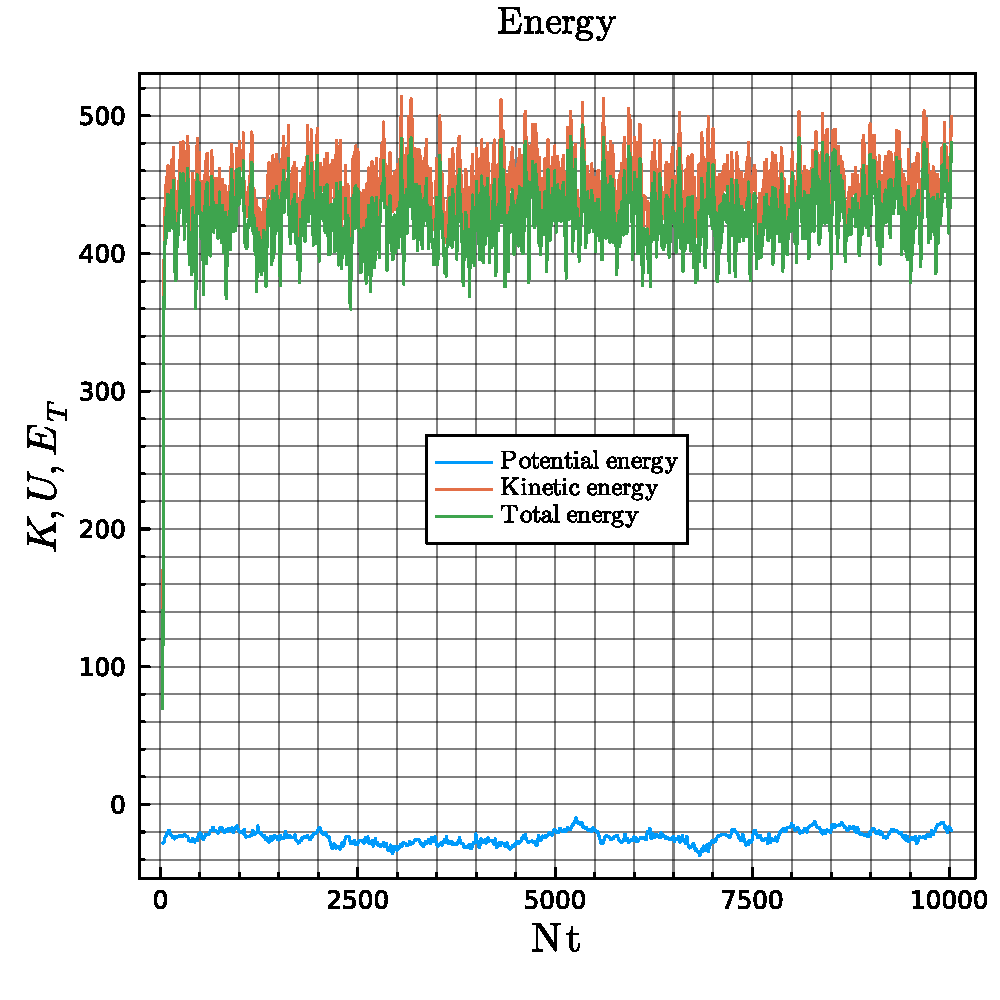
\includegraphics[width=0.65\textwidth]{imgs/hw3/energy.pdf}
    \caption{Potential, kinetic and total energy of the binary fluid.}
    \label{fig:energy}
\end{figure}





\end{document}